\subsection{Banco de atenuadores y aisladores N2002A (Noise Source Test Set )}
El banco de atenuadores y aisladores N2002A (figura \ref{Fig:BancoAtenuadoresAisladores}) es un dispositivo que, de acuerdo a la nota de aplicación de Agilent Technologies \cite{AGI02}, esta destinado a facilitar la calibración de fuentes de ruido de forma rápida y precisa. Es un instrumento que se integra a un sistema para calibración de fuentes de ruido, como el mostrado en la figura \ref{Fig:BancoPruebasFuenteRuido}. 		

\begin{figure}[h!]
	\centering
	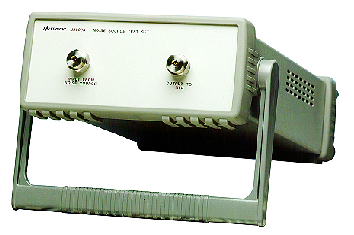
\includegraphics[height=6cm]{./Imagenes/BancoAtenuadoresAisladoresN2002.pdf}
	\caption{Interfaces eléctricas del N2002A}			
	\label{Fig:BancoAtenuadoresAisladoresN2002.pdf}
\end{figure}

En la medición de figura de ruido de alta precisión la incertidumbre de esta esta fuertemente relacionada a la incertidumbre de la fuente de ruido empleada en la medición. Al conformar un banco de calibración de NS empleando el N2002A, se pueden realizar mediciones de alta precisión en “casa”, lo que evita recurrir a laboratorios especializados	para efectuar esta tarea.

se debe emplear cuando se efectúan mediciones de ENR alta precisión en fuentes de ruido.

El N2002A se inserta en el camino de señal de RF o UW, entre la salida de la fuente de ruido bajo prueba y la entrada	del NFA. La función de este es de proveer aislamiento entre la fuente de ruido y el NFA con el fin de minimizar el	coeficiente de reflexión. Las reflexiones entre el DUT y la fuente de ruido causan incertidumbre en la potencia de ruido que emerge de la fuente; la medición entonces no se refiere a la impedancia de 50 Ohms deseados, sino a la impedancia actual de la fuente de ruido. Incorporando el N2002A dentro del sistema de calibración se minimiza la interacción entre el DUT y el NFA, minimizando el coeficiente de reflexión y de esta forma la incertidumbre. Esto
permite una calibración más precisa de la fuente de ruido, asegurando precisión, repetibilidad y trazabilidad en las	mediciones ademas de reducir de manera significativa la incertidumbre [2].	

En la figura \ref{Fig:VistaInternaN2002} se muestra una vista interna y en la figura \ref{Fig:EstructuraInternaN2002} una vista esquemática de la estructura interna del dispositivo. Se aprecia que este equipo esta conformado por cuatro secciones de atenuadores y una sección de aislador. Los atenuadores o el aislador son conectados o desconectados del camino de señal por medio dos conjuntos de interruptores, etiquetados como A2 y A6 respectivamente en la figura 3. Las señales que controlan estos interruptores provienen del exterior del equipo, son generadas por un dispositivo de la serie 11713 de Agilent / Keysight Technologies, unidad controladora de atenuadores e interruptores. Cada sección de atenuador permite el paso de señal en un rango de frecuencia distinto,
como se indica en la figura 3. El N2002A cubre un rango de frecuencias idéntico al del N8975, va desde \SI{10}{\mega\hertz} MHz hasta \SI{26.5}{\giga\hertz}. 

\begin{figure}[h!]			
	\centering
	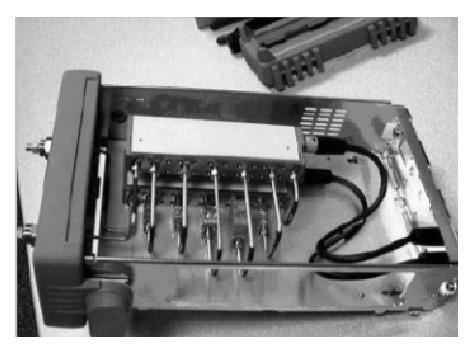
\includegraphics[width=15cm]{Imagenes/VistaInternaN2002.pdf}
	\caption{Esquema de la estructura interna para el N2002S}
	\label{Fig:VistaInternaN2002}
\end{figure}

El N2002A no posee fuente de poder interna ni tampoco realiza mediciones. No dispone de interfaz de usuario, este equipo debe ser comandado por medio de un dispositivo de la serie 11713. EL 11713 brinda la interfaz de usuario necesaria, en	éste el usuario realiza la selección del rango de frecuencia sobre el cual N2002A debe permitir el paso.		

El N2002A cuenta únicamente con interfaces eléctricas dispuestas en el panel frontal y posterior del equipo (figura \ref{Fig:InterfacesElectricasN2002}). La interfaz para señal de RF / UW esta dispuesta en el panel frontal (figura	\ref{Fig:InterfacesElectricasN2002}a) y posee dos conectores, un conector es la entrada de señal en el cual se conecta la fuente de	ruido (izquierda) y el otro conector es la salida filtrada o atenuada la cual se conecta a la entrada de señal del NFA (derecha). En en el panel posterior se encuentra la interfaz para señales de control (figura \ref{Fig:InterfacesElectricasN2002}b), en esta se encuentran dos conectores para las señales generadas por un dispositivo de la serie 11713.		

\begin{figure}[h!]
	\centering
	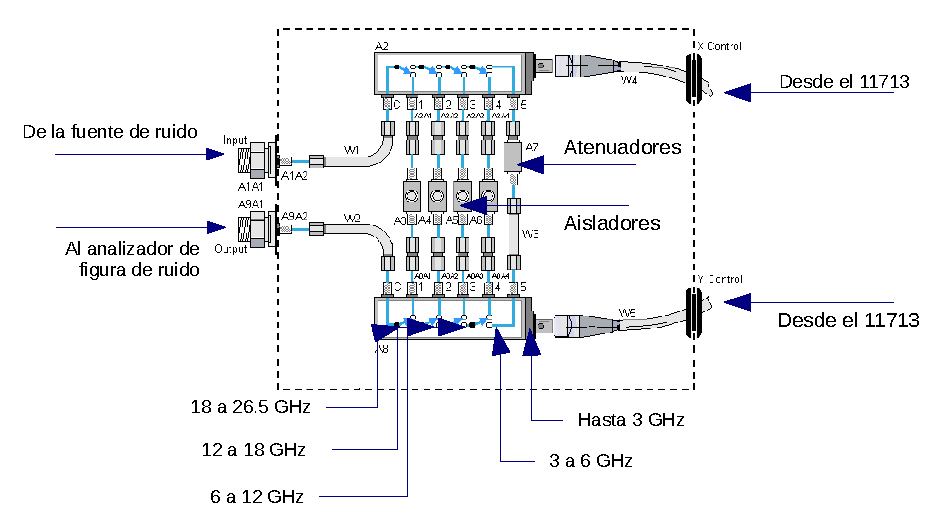
\includegraphics[width=15cm]{Imagenes/EsquemaEstructuraInternaN2002.pdf}
	\caption{Esquema de la estructura interna del N2002A}			
	\label{Fig:EsquemaEstructuraInternaN2002}
\end{figure}

\begin{table}[h!]
	\centering
	\begin{tabular}{cccc}
		\toprule
		A1 & Aislador 18 \si{\giga\hertz} – 26,5 \si{\giga\hertz} \\
		\midrule
		A2 & Aislador 12 \si{\giga\hertz} – 18 \si{\giga\hertz} \\
		\midrule
		A3 & Aislador 6 \si{\giga\hertz} – 12 \si{\giga\hertz} \\
		\midrule
		A4 & Aislador 3 \si{\giga\hertz} – 6 \si{\giga\hertz} \\		
		\midrule
		A5 & Atenuador 3 \si{\decibel} \\				
		\bottomrule
	\end{tabular}
	\caption{Rangos de ENR nominal para fuentes de ruido serie N4000}
	\label{Tab:RangosFuentesRuido}
\end{table}

\begin{figure}[h!]
	\centering
	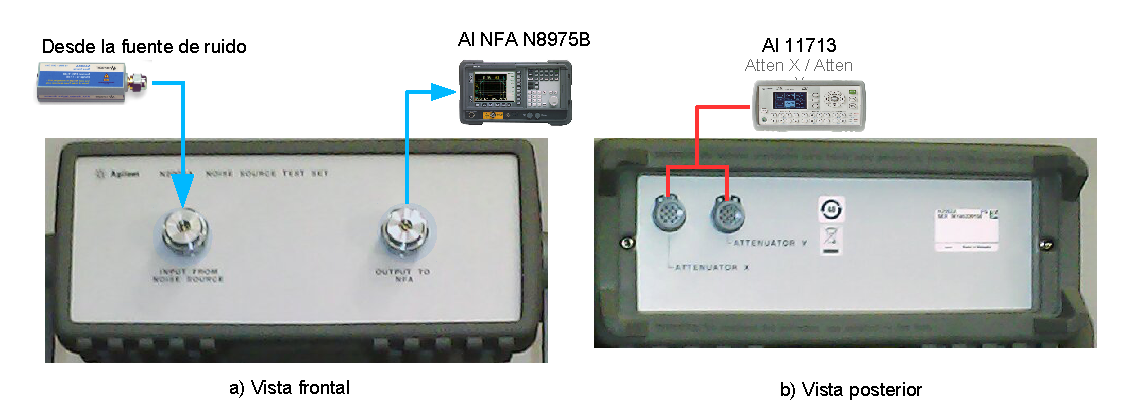
\includegraphics[width=16cm]{Imagenes/InterfacesElectricasN2002.pdf}
	\caption{Esquema de la estructura interna del N2002A}			
	\label{Fig:InterfacesElectricasN2002}
\end{figure}

Según recomendación de Agilent, se debe usar el N2002A en conjunto con el Agilent N8975A (NFA) como equipo básico fundamental para calibración de fuente de ruido. N2002A es un equipo para calibrar fuentes de ruido “en casa” [3.3]. El objetivo es calibrar fuentes de ruido a estándar trazables.

Permite calibrar de manera rápida, repetible con niveles mínimos de incertidumbre. Este equipo es necesario cuando se	realizan pruebas de ENR sobre una fuente de ruido. Asegura resultados de calibración precisos, incrementa la confianza en la medición, permite el desarrollo de DUTs con especificaciones más exigentes. Entrega resultados trazables a 	estándares nacionales.

\begin{figure}
	\centering
	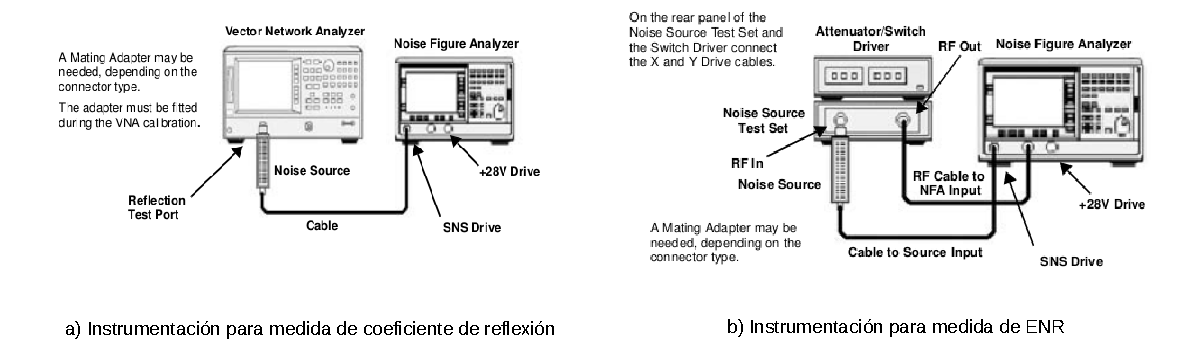
\includegraphics[width=5cm]{Imagenes/InstrumentacionCalibracionN2002.pdf}
	\caption{Instrumentación para calibración de fuentes de ruido}
	\label{Fig:InstrumentacionCalibracionN2002}
\end{figure}

El proceso de calibración consiste en comparar el desempeño de forma trazable de una fuente de ruido en relación al desempeño de otra fuente de ruido, que se toma como estándar de calibración, o contra las especificaciones del fabricante. Para ello se realizan \ dos pruebas de verificación de desempeño: 

\begin{itemize}
\item Medición de la razón de ruido excedente (ENR).
\item Medición del coeficiente de reflexión complejo (magnitud y fase). 
\end{itemize}

Si la fuente de ruido falla cualquiera de estas pruebas es indicador que requiere reparación o ajuste.

El sistema de calibración de Agilent permite verificas las fuentes de ruido Agilent de la serie 346 (346A, 346B, 346C) y las fuentes de ruido inteligentes de la serie Agilent N4000A (N4000A, N4001A, N4002A). Este proceso de calibración permite calibrar fuentes de ruido entre \SI{10.0}{\mega\hertz} y \SI{26.5}{\mega\hertz}. 

En la figura \ref{Fig:InstrumentacionCalibracion} se muestra la instrumentación propuesta por Agilent \cite{AGI03} para la medida de coeficiente de reflexión (figura \ref{Fig:InstrumentacionCalibracion}a) y para la medida del ENR (figura \ref{Fig:InstrumentacionCalibracion}b).	

\begin{table}
	\centering
	\begin{tabular}{m{6cm}m{6cm}}
		\toprule
		\textbf{Coeficiente de reflexión} 	&	\textbf{ENR}	\\
		\midrule
		Analizador de red que cubra el rango 10 \si{\mega\hertz} a 26.5 \si{\giga\hertz} (VNA) 8753ES o 8753ET, 8722ES o 8722ET 	&	Analizador de figura de ruido N8975A \\
		\midrule
		Analizador de figura de ruido N8975A	&	N2002A conjunto para pruebas con fuentes de ruido \\
		\midrule		
		Kit de calibración para VNA			&	Controlador de atenuadores e interruptores 11713 \\
		\midrule		
		Controlador de atenuadores e interruptores 11713	& 	Fuente de ruido referencia estandar \\
		\midrule		
		Cable Viking para conexión del 11713	&	\\
		\bottomrule		
	\end{tabular}
\end{table}

\subsection{Descripción de las pruebas de verificación}
\subsubsection{Medición de ENR}
La prueba de ENR consiste en comparar los resultados de la prueba sobre una fuente de ruido bajo prueba (DUT) contra los	resultados de una prueba sobre una fuente de ruido referencia estándar. La referencia estándar es una fuente de ruido calibrada con valores conocidos de ENR. Las medidas se llevan a cabo tanto en la fuente de ruido DUT asi como en la fuente de ruido referencia estándar. Los valores de ENR del DUT se derivan de estos resultados. 

Los resultados de esta prueba permiten asegurar si la fuente de ruido cumple con las especificaciones de calibración del fabricante. La precisión de la medidas para el DUT es altamente dependiente de la exactitud de la calibración de la referencia estándar. Se debe usar, según Agilent, una referencia estándar que haya sido calibrada por un laboratorio especializado.

Las pruebas deben realizarse dentro de la temperatura ambiente de 296 ± 1K (23 ± 1) °C.

Las fuentes de ruido requieren calibración periódica del desempeño operacional. En condiciones de uso normal y ambientales, se calibra la NS cada 12 meses [1.27].

\subsubsection{Resumen del procedimiento de medición de ENR [1.29] [1.39].}
Se emplea la instrumentación indicada en la figura \ref{seq:refDrawing4}b. Se inicia el proceso al encender los equipos y permitir que calienten por una hora. Se debe permitir que las fuentes de ruido se estabilicen a la temperatura	ambiente. No se deben usar las fuentes de ruido una hora antes de realizar las mediciones.
	
Se deben cargar los datos de ENR de la fuente de ruido referencia estándar en el analizador de figura de ruido. Estos datos los proporciona el fabricante de la NS ya sea en formato digital o físico. SI se usa una fuente de ruido inteligente (SNS), el NFA puede cargar los datos de ENR que se encuentran en la memoria de la SNS de forma automática, si el NFA esta habilitado.

La secuencia de pasos para la medición emplea las tabla \ref{seq:refDrawing5}a para registro de resultados

\begin{itemize}
\item Los valores de ENR de la referencia estándar (ENR1) son conocidos, ingresar estos valores en la columna ENR1 de la
tabla 1.
\item Se conecta el equipo de prueba como indica la figura \ref{seq:refDrawing4}b.. Conectar la fuente de ruido de
referencia, asegurando que el conector RF de esta NS es del mismo tipo que el conector de la NS DUT]. Ajustar los
interruptores del 11713, para el canal de frecuencia requerido, por ejemplo interruptores 9 y 0 ON para medir entre
10MHz y 3.0GHz. 
\item Establecer el equipo para realizar la medida del primer punto de frecuencia. 
\item Medir el factor Y lineal de la NS referencia estándar.
\item Anotar este valor en la tabla , bajo la columna Y1.
\item Establecer el equipo para medir el siguiente punto de frecuencia, repetir el procedimiento hasta que todos los
puntos de medición estén completos.
\item Remover la referencia estándar de la entrada del N2002A y la NS DUT.
\item Establecer el equipo para medir el primer punto de frecuencia.
\item Medir el factor Y lineal en la NS DUT.
\item Anotar en las tablas de registro el resultado bajo la columna Y2.
\item Repetir el procedimiento para todos los puntos a medir.
\item Con los resultados obtenidos, introducirlos en las ecuaciones y calcular con ellas el ENR y los valores de
incertidumbre.
\end{itemize}

Conectar cables Viking de la parte posterior del 11713A a la parte posterior del N2002A. Conectar Atten X del 11713A al Attenuator X del N2002A. Conectar Atten Y del 11713A al Attenuator Y del N2002A.

Proceso de Calibración [1.26]	
SI la fuente de ruido falla cualquiera de estas pruebas de desempeño, la NS requiere reparación.

Aparte de la calibración en puntos cardinales de frecuencia, se puede realizar la calibración en otros puntos. El máximo de puntos frecuencia-ENR es de 81.
	
Tabla de VSWR típico en [1.19]

Agilent N2002A empleado cuando se requiere realizar pruebas de Razón de Ruido en Exceso (ENR) sobre una fuente de ruido [1.14]. 

\subsubsection{Ecuaciones}
\emph{ENR}
\begin{equation}
	ENR_2 = 10\log\left(\frac{\left(Y_2-1\right)\left(T_0\frac{10^\frac{ENR_1}{10}}{Y_1-1}\right)}{T_0}\right)
\end{equation}

\emph{Incertidumbre}
\begin{equation}
	U_{C}ENR_2=\sqrt{(U_{C}ENR_1)^2+(U_{C}Sys)^2}
\end{equation}

donde

TO = 290 K.

ENR1 = Valor de ENR de la fuente de ruido de referencia en cada punto de frecuencia.

ENR2 = Valor calculado de ENR de la fuente de ruido DUT en cada punto de frecuencia.

Y1 = Valor medido del factor Y de la fuente de ruido de referencia en cada punto de frecuencia.

Y2 = Valor medido del factor Y de la fuente de ruido DUT en cada punto de frecuencia.

UcENR1 = Valor de incertidumbre de ENR de la fuente de ruido de referencia en cada punto de frecuencia.

UcENR2 = Valor calculador para la incertidumbre de ENR de la fuente de ruido de referencia en cada punto de frecuencia.

UcSys = Incertidumbre total del sistema de medición en cada punto de frecuencia.

	
\begin{figure}[h!]
\centering
 Tablas para registro
	de datos, relativos a la medición de ENR
\end{figure}

El N2002A es controlado por el 11713A. El 11713A es controlado por el software N2002A Noise Source Demonstration Software (No encontrado. Ver en su lugar VEE PRO en KeySight).

Equipo de Prueba Recomendado

Para mediciones de ENR y el coeficiente de reflexión (magnitud \ y fase), equipo listado en las tablas 2-4 y 2-5 del
documento [1].		

\subsection{Medición de coeficiente de reflexión (magnitud y fase) [1.31]}
\subsection{Rango de las mediciones de ENR para fuentes de ruido Agilent}
La medición de ENR sobre la fuente de ruido permite garantizar que esta se encuentre dentro de las especificaciones, por ejemplo dadas por Agilent en la tabla 1.		

Automatización del proceso de medición

El software que automatiza el proceso de medición esta escrito dentro de Agilent VEE Pro, el cual parece ser un entorno de ejecución (run time), esta disponible como un archivo VEE Pro o un archivo VEE Pro run time (posiblemente sea un script). 

\begin{itemize}
\item Software listado en [3.8]
\item Agilent VEE Pro
\item Agilent VEE Pro run time (provisto con el N2002A)
\end{itemize}
VEE Pro puede comunicarse a través de GPIB, LAN, USB, RS-232, VXI y LXI.

Para su uso requiere una tarjeta de interfaz GPIB (Agilent o National Instruments).

Sistema de calibración de fuente de ruido Agilent		

El sistema de la figura 1 cuenta con los equipos [2.5]:

\begin{itemize}
\item NFA N8975, opera en un rango de 10MHz a 26.6GHz) (con opción 1D5 la cual es una referencia de frecuencia de alta
estabilidad). 
\item Cuenta con el N2002A conjunto para pruebas con fuente de ruido que puede incluir todos los cables y conectores
necesarios para ejecutar calibración de NS con conectores de 3.5mm y tipo N (opción 001). Incluye el 11713A. 
\item Incluye una fuente de ruido estándar de oro.
\end{itemize}
Características del sistema [2.5]

Entre otras, puede calibrar fuentes de ruido tipo SNS y de la serie 346 de Agilent.

Nota importante de [2.3]

El N2002A conjunto para pruebas con fuente de ruido debe ser usado en un sistema de calibración de fuente de ruido, este
equipo no posee fuente de poder y no realiza mediciones.

\subsection{Equipo complementario al N2002A}
Según [2.4] este equipo cuenta con las fuentes de ruido inteligentes (SNS) Agilent de la serie N4000 y de la serie 346.

\subsection{Prueba de verificación [1.17]}
Por medio de un analizador vectorial de red se verifica el coeficiente sea el que indica la tabla para cada frecuencia.

\begin{table} 
	\begin{tabular}{ccc}
		\toprule
		\textbf{Frecuencia(\si{\giga\hertz})} & \textbf{Límite ROE \newline típico} & \textbf{Combinación \newline de botones 11713} \\
		\midrule
		0.01 	&	1:1.05	&	0 On, 9 On \\
		0.1 	&	1:1.05	&	0 On, 9 On \\
		1	 	&	1:1.05	&	0 On, 9 On \\
		2 		&	1:1.05	&	0 On, 9 On \\
		3 		&	1:1.05	&	0 On, 9 On \\
		4 		&	1:1.1	&	1 On, 5 On \\
		5 		&	1:1.1	&	1 On, 5 On \\
		6	  	&	1:1.1	&	1 On, 5 On \\
		7	 	&	1:1.15	&	3 On, 7 On \\
		8	 	&	1:1.15	&	3 On, 7 On \\
		9	 	&	1:1.15	&	3 On, 7 On \\
		10	 	&	1:1.15	&	3 On, 7 On \\
		11	 	&	1:1.15	&	3 On, 7 On \\
		12	 	&	1:1.15	&	2 On, 6 On \\
		13	 	&	1:1.15	&	2 On, 6 On \\
		14	 	&	1:1.15	&	2 On, 6 On \\
		15	 	&	1:1.15	&	2 On, 6 On \\
		16	 	&	1:1.15	&	2 On, 6 On \\
		17	 	&	1:1.15	&	2 On, 6 On \\																																				
		18	 	&	1:1.15	&	2 On, 6 On \\
		19	 	&	1:1.18	&	4 On, 8 On \\
		20	 	&	1:1.18	&	4 On, 8 On \\
		21	 	&	1:1.18	&	4 On, 8 On \\
		22	 	&	1:1.18	&	4 On, 8 On \\
		23	 	&	1:1.18	&	4 On, 8 On \\								
		24	 	&	1:1.15	&	4 On, 8 On \\
		25	 	&	1:1.18	&	4 On, 8 On \\
		26	 	&	1:1.18	&	4 On, 8 On \\
		26.5 	&	1:1.18	&	4 On, 8 On \\	
		\bottomrule	
	\end{tabular}
\end{table}




